
\chapter{Automatická tvorba grafu kontaktů}\label{Grafy_kontaktu}

\textit{Milan Zajíček, Karel Vrbenský}
\vspace{15mm}

\section*{Úvod}

Obvykle užívaný model epidemie SIR (Susceptibles, Infectives, Removed, tedy potenciálně vnímaví, infekční a vyčlenění ze struktury) obsahuje jako vstupní podmínky počty jedinců z~těchto skupin a predikuje přírůstky či úbytky v~každém časovém kroku. Epidemickými parametry jsou přitom hodnoty jako například míra infekčnosti, míra uzdravení atd., které určují intenzitu, se kterou dochází k~přechodům mezi stavy. Chování jednotlivců je u~tohoto modelu zahrnuto právě do intenzit těchto přechodů. Matematickým modelům epidemie se věnuje kapitola \ref{Typy_modelu}. Chceme-li modelovat šíření epidemie na úrovni jednotlivých kontaktů individuálně definovaných jedinců, je třeba vytvořit strukturu obsahující všechny jednotlivce a jejich vzájemné vazby. Tuto strukturu nazýváme graf kontaktů. V~grafu jsou jednotlivci reprezentováni jako uzly s~definovanými vlastnostmi, jejich kontakty pak představují hrany. Mezi významné atributy hran patří intenzita (počet kontaktů v~čase) a pra\-dě\-po\-dob\-nost přenosu nákazy při konkrétním setkání. 

Graf kontaktů získáváme vlastním generátorem, vytvořeným pro softwarový ná\-stroj EPICITY, což je program umožňující testovat vliv protiepidemických opatření v~rám\-ci regionu. Rigorózně je náš postup popsán v publikaci \cite{M-techrep2021}.

Výhodou použití grafu diskretizovaného na úroveň jednotlivců je proti SIR modelu především možnost modelovat průběh epidemie s~vysokou granularitou. Je možné sledovat rychlost šíření nákazy dle nejrůznějších kritérií, například z~hlediska geografie, podle věkových kohort, ekonomických aktivit atd.  Jiným možným příkladem je simulace výskytu superpřenašeče v~nějakém místě či v~určité komunitě, jehož simulace v~SIR modelu není možná.
Graf kontaktů může být navržen jako vícevrstvá struktura, ve které jednotlivé vrstvy představují specifickou třídu kontaktů. 


Těchto vrstev získáváme přibližně třicet a odpovídají setkáním v~rodině, práci, škole, restauracích atd.

Při tvorbě grafu vycházíme z~dat, která poskytují sociologické výzkumy \cite{paqcovid, zaj:mediancovid, zaj:medianlife}, Český statistický úřad,\footnote{https://www.czso.cz} Katastrální úřad,\footnote{https://cuzk.cz} a openstreetmap.\footnote{https://www.openstreetmap.org} Velké množství anonymizovaných dat pro tvorbu grafu poskytla bezplatně společnost Seznam.cz, a.s., služba Firmy.cz.\footnote{https://www.firmy.cz/}

Tento článek se zabývá pouze tvorbou grafu kontaktů, tedy zdroje informací pro simulace, jimiž se podrobně zabývají texty kapitoly \ref{Agentni_modely}, v~nichž lze najít obecný popis modelu, a kapitoly \ref{Evaluace_politik} obsahující konkrétní příklady použití modelu pro srovnání různých experimentálních scénářů průběhu epidemie.

\section*{Konstrukce grafu kontaktů}

První námi konstruovaný graf vycházel z~geograficky definovaného středně velkého regionu a sloužil pro vytvoření metodiky použitelné pro libovolný region ČR. Pracoval s~městem Hodonín s~24 tisíci obyvatel a okolními obcemi, v~nichž žije dalších 32 tisíc lidí. Vzniklá síť představovala 2,8 milionu potenciálních kontaktů. 

Základním zdrojem pro zjištění struktury obyvatelstva jsou data Českého statistického úřadu (ČSÚ) získaná při sčítání lidu v~roce 2011. Tato data obsahují informace o~věku, pohlaví, místě pobytu, typu domácnosti a počtu členů domácnosti. Dalším druhem dat, která v~tomto ohledu vstupují do modelu, jsou informace o~hustotě zalidnění, tedy geometrické souřadnice jednotlivých domů doplněné o~počty bytů. Jelikož data nejsou vzájemně provázána, nezbývá než přiřazovat bydliště jednotlivcům náhodně. Dostupná data rovněž nejsou personalizována. Z~tohoto faktu vyplývá nutnost rozdělit populaci do domácností tak, aby obsazenost jednotlivých bytů a domů odpovídala nejen počtu domácností, ale také věkové struktuře členů domácností podle sčítání lidu. Algoritmus rozdělování lidí do domácností respektuje jak věkovou skladbu, tak další skutečnosti, jako je například vícegenerační bydlení v~rodinných domech.

Každému ednotlivci je v~grafu náhodně přisouzen druh ekonomické aktivity v~závislosti na věku a pohlaví tak, aby výsledný profil všech jednotlivců odpovídal agregovaným datům o~struktuře zaměstnanosti v~daném regionu. S~věkem souvisí i přiřazení jednotlivých osob do školní výuky, obdobně jako například přiřazení osob důchodového věku mezi osoby trávící většinu času v~domácnosti. Každá osoba je tedy definována svými sociologickými charakteristikami (věk, pohlaví, druh ekonomické aktivity atd.) a rozdělení těchto vlastností v~celé populaci odpovídá údajům ze sčítání lidu v~roce 2011. Pro ilustraci: v~grafu můžeme nalézt například třiačtyřicetiletého ekonomicky aktivního učitele, pracujícího v~místě bydliště, žijícího s~manželkou a třemi dětmi v~rodinném domě. Dotyčný má 12 přátel, se kterými se pravidelně potkává, většina z~nich je jeho věku, každý den cestuje hromadnou dopravou do zaměstnání a pravidelně navštěvuje rodiče v~blízké vesnici.

Lidé navazují řadu kontaktů, ať již pravidelných a predikovatelných, anebo zcela náhodných v~čase i prostoru. 
%Vědecké uchopení této skutečnosti, zvláště má-li být definována míra kontaktu, je z matematického pohledu velmi složité. Určení hodnoty pravděpodobnosti setkání dvou lidí je úkol, jehož řešení závisí na řadě parametrů, které jsou v mnoha případech těžko kvantifikovatelné.
Některé kontakty lze odhadnout z~podstaty věci, například kontakty v~rámci rodiny a ve škole, kam musí chodit každé dítě školního věku. Ostatní se odhadují hůře, a proto používáme kontaktní matice dostupné v~literatuře \cite{Prem_etal2017}, ze sociologických výzkumů anebo expertních odhadů. 
U~každého kontaktu je důležitá jeho intenzita. Obr. \ref{kategorie} ukazuje v~levém sloupci porovnání středních počtů kontaktů ve vrstvách, zatímco v~pravém sloupci jsou znázorněny pravděpodobnosti nakažení ve vrstvách tak, jak byly vypočítány během tvorby grafu kontaktů.
%Z dat a literatury, kterou máme k dispozici, je možné realisticky určit pouze některé druhy kontaktů, v našem modelu jsou to kontakty v rodinách a kontakty ve škole. Pro ostatní druhy kontaktů (zaměstnání, přátelské kontakty a specificky kontakty v restauracích) je třeba pracovat s odhady založenými na sociologických výzkumech. Z těch je zajisté možné získat informace o tom, jak často lidé z konkrétní věkové skupiny navštěvují restaurace, nebo jaké procento populace holduje tomu kterému sportu, ovšem relevantní informace o tom, jak intenzivní jsou například kontakty v případě tréninku házené ve srovnání s tréninkem kanoistů, již oporu v datech hledají těžko. Pokud je to možné, používáme tedy jako parametry dohledatelná a vědecky podložená data. V případě, že taková data k dispozici nejsou, používáme expertních odhadů, jako například při určování kapacit obchodů a množství návštěvníků obchodních center. Tímto způsobem můžeme například získat představu o vztahu mezi počtem kontaktů v určité skupině kontaktů a počtu nakažlivých osob v nich, jak je uvedeno na obr.\ref{kategorie}. 

%Hodnoty vah pro množství infekčních osob byly získány Saatyho metodou, dotazníkovým šetřením mezi experty.

Pravděpodobnosti nakažení v~jednotlivých prostředích se přirozeně liší, například při blízkém fyzickém kontaktu v~uzavřené místnosti budou jiště větší než při venkovní sportovní aktivitě. Odhady těchto pravděpodobností jsme získali dotazníkovým šet\-ře\-ním mezi experty, které jsme vyhodnotili Saatyho metodou \cite{M-techrep2021}.

\begin{figure}
    \centering
    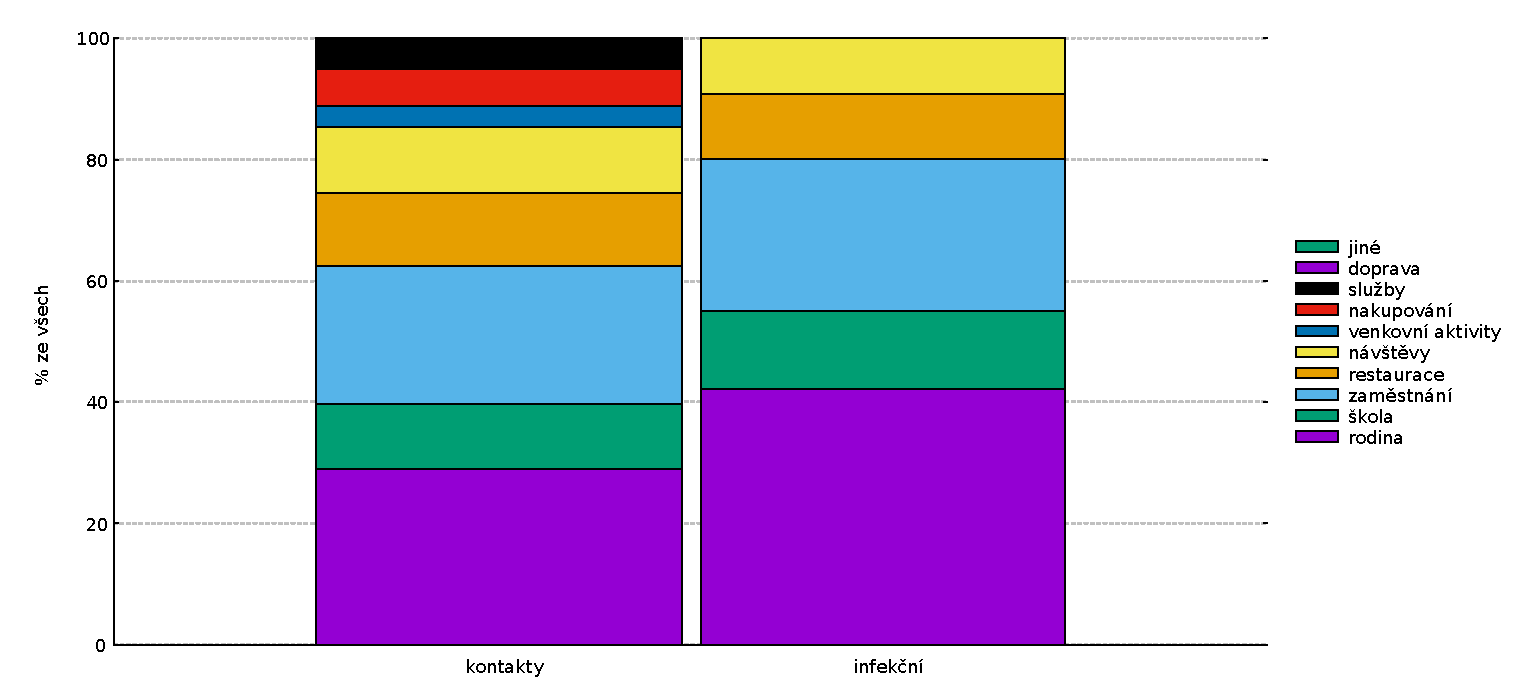
\includegraphics[width=11cm]{pic/filled_cz.eps}
    \caption{Poměr počtu kontaktů a infekčních osob v~jednotlivých kategoriích kontaktů.}
    \label{kategorie}
\end{figure}

Jak bylo již naznačeno, kontakty rozdělujeme do následujících kategorií: kontakty v~rodině, kontakty ve škole, kontakty na pracovišti a kontakty při volnočasových aktivitách, mezi které patří například návštěvy restaurací, návštěvy v~jiných domácnostech, nebo návštěvy divadel atd. Vlastní přístup ke tvorbě grafu kontaktů vy\-ža\-du\-je také doprava či setkávání během nakupování. Způsob tvorby vrstev grafu je podrobně popsán v~\cite{M-techrep2021}, kde jsou vysvětleny postupy vedoucí k~určení jednotlivých parametrů včetně odůvodnění. Dále popíšeme implementaci kontaktů ve vybraných vrstvách grafu kontaktů.

Jak je uvedeno výše, pro tvorbu \emph{rodinných kontaktů} využíváme anonymizovaných dat ČSÚ, která umožňují modelovat jednotlivě každou domácnost. Předpokládáme, že se každý člen domácnosti setkává se všemi jejími ostatními členy. Dále se potkávají členové různých domácností v~rámci stejného bydliště (domu). Posledním zdrojem kontaktů v~rámci domácností jsou pak mezigenerační návštěvy.
Každou osobu starší 50 let považujeme za potenciálního rodiče, který bude navštěvovat domácnosti svých dětí. Počet dětí získáváme z~cenzurovaného normálního rozdělení s~průměrem 1,92 a standardní odchylkou 0,7. Tyto hodnoty odpovídají údajům z~výzkumu \cite{zaj:ess}.

Domácnost dětí je volena náhodně tak, aby alespoň jeden člen domácnosti byl ve věku rodičů (prarodičů) minus 20 let.

Při těchto mezigeneračních návštěvách se předpokládá, že daný rodič se při návštěvě svých dětí setkává se všemi členy jejich domácností. Podobně také děti navštěvují své rodiče a při té příležitosti se mohou setkat se všemi členy domácnosti rodičů.

Pravděpodobnosti jednotlivých typů kontaktů (v~rámci domácnosti, me\-zi\-ge\-ne\-rač\-ní) jsou během vytváření grafu automaticky optimalizovány tak, aby odpovídaly matici kontaktů pro rodinné prostředí tak, jak je uváděna v~práci \cite{Prem_etal2017}. Kritériem pro optimalizaci je 
minimalizování vážené kvadratické vzdálenosti výsledné matice kontaktů a matice kontaktů pro domácnosti z~\cite{Prem_etal2017}.

%Chceme-li respektovat matici kontaktů pro rodinné prostředí tak, jak je uváděna v literatuře \cite{Prem_etal2017}, musíme určit pravděpodobnosti kontaktů u jednotlivých věkových skupin, jak je podrobně rozebráno v \cite{pg:modelM}. Například u seniorů a osob obdobného věku je tato pravděpodobnost nastavena na 1 -- a to v případě, že je dotyčným osobám více než 60 let, anebo je jejich věkový rozdíl menší či roven 10 letům. V ostatních případech je hodnota pravděpodobnosti kontaktu v rodině nastavena na 0,745. V případě domácností, ve kterých žijí dvě rodiny, předpokládáme kontakt se kterýmkoli členem druhé rodiny s pravděpodobností 0,397.

%Dalším předpokladem pro tvorbu kontaktů v rodinách je skutečnost, že každá osoba starší 50 let navštěvuje domácnosti svých dětí. Počet těchto kontaktů získáváme z cenzurovaného normálního rozdělení s průměrem 1,92 a standardní odchylkou 0,7, kteréžto hodnoty odpovídají údajům z výzkumu \cite{zaj:ess}.
%Žijí-li v domácnosti dvě nebo více osob starších 50 let, předpokládáme jejich kontakt s domácnostmi jejich dětí. Jako takové jsou náhodně voleny domácnosti, ve kterých je alespoň jeden člen ve věku rodičů (prarodičů) minus 20 let. Starší navštěvují mladší s pravděpodobností 0,297 dělenou počtem dětí (věnují se všem dětem rovnoměrně). Naopak děti navštěvují své rodiče s pravděpodobností 0,373. Při každé takové návštěvě se předpokládá kontakt se všemi členy domácnosti. Uvedené pravděpodobnosti jsou stanoveny minimalizováním vážené kvadratické vzdálenosti výsledné matice kontaktů a matice kontaktů pro domácnosti z \cite{Prem_etal2017}.


Pro určení \emph{kontaktů ve školách} poskytlo důležitý zdroj informací Ministerstvo školství ČR, které provozuje volně přístupnou databázi školských zařízení. Databáze obsahuje informace o~umístění a kapacitě všech druhů školských zařízení v~ČR \cite{zaj:skolskazarizeni}. Jelikož databáze obsahuje i kapacity škol, lze přiřadit děti podle věku do mateřských škol, základních škol (včetně rozdělení na první a druhý stupeň), středních škol a škol vysokých, s~ohledem na demografický profil regionu. V~případě Hodonínska, které nemá žádnou vysokou školu, jsou starší studenti osobami, které z~regionu za studiem vyjíždějí.

Přidělování žáků do jednotlivých škol probíhá takto: Seznam žáků je náhodně promíchán a žáci jsou postupně přidělováni do nejbližší školy, a to až do okamžiku, než se naplní její kapacita. Po naplnění kapacity škol jsou následně žáci podle věku rozděleni do jednotlivých ročníků a dále do tříd tak, aby v~každé třídě bylo maximálně 20 studentů. Ke každé třídě je přidělen jeden třídní učitel, například právě ten, který byl zmíněn o~několik odstavců výše. 
%Nejprve jsou prohledáni učitelé ze stejné obce, a pokud již není žádný k dispozici, vybere se náhodně z učitelů, jejichž doba dojezdu do školy je kratší než 30 minut. Poté, co jsou určeni třídní učitelé, je do každé školy umístěno ještě dvakrát více učitelů bez třídnictví. 
Uvažujeme následující typy kontaktů: mezi žáky v~rámci třídy, mezi žáky v~rámci celé školy, mezi učiteli i žáky v~rámci celé školy a konečně mezi všemi učiteli školy navzájem.
Podobně jako u~rodinných kontaktů se pravděpodobnosti pro vygenerovaný graf kontaktů optimalizují tak, aby odpovídaly matici kontaktů pro školy z~\cite{Prem_etal2017}.


%Ve školách, obdobně jako v restauracích či obchodech, dochází mezi studenty a učiteli i k náhodnému setkávání, které je třeba rovněž zahrnout do modelu.

\emph{Kontakty na pracovišti} jsou vytvářeny na základě odhadu údajů o~ekonomické aktivitě obyvatelstva a zastoupení pracovních odvětví v~regionech. Osobám v~produktivním věku jsou zaměstnání přidělena tak, aby respektovala zastoupení každého druhu pracovní činnosti (zemědělství, průmysl, obchod, doprava, IT atd.) s~ohledem na charakteristiku regionu podle dat ČSÚ. Při tvorbě kontaktů na pracovišti lze předpokládat intenzivní setkávání v~rámci jednoho odvětví. Respektovat je však třeba i rozdílnou míru setkávání napříč odvětvími. Počty kontatků mezi sektory, případně s~klienty jsou určovány podle matice počtu vzájemných pracovních kontaktů pro různé obory činnosti \cite{Prem_etal2017}. Některé pracovní kontakty jsou určeny explicitně, ať již z~povahy práce, anebo díky expertním znalostem, například kontakty ve školách, kontakty v~restauracích, kontakty v~obchodech atd.

% následující odstavec do dopravy
% Pracovní kontakty vytvářejí rovněž požadavky na dopravní síť. Jelikož jsou známy časy, které lidé tráví cestou do práce, je možné osoby do zaměstnání dopravovat i s ohledem na dobu cestování známou ze sociologických výzkumů.

% \emph{Kontakty na pracovišti} jsou v našich modelech díky znalostem o průběhu pracovního procesu explicitně definovány pro učitele, zaměstnance restaurací a prodavače. Tato povolání však tvoří pouze přibližně 4\,\% pracující populace. Pro zbývající odvětví je intenzita pracovních kontaktů odhadnuta ze sociologických výzkumů. Zaměstnanci jsou přiděleni do obcí tak, aby respektovali rozdělení odvětví, jak je známe z dat ČSÚ (zemědělství, průmysl, obchod, doprava, IT atd.). Podle počtu pracovníků na každém pracovišti je (obdobně jako v případě škol) určena intenzita kontaktů, a to za předpokladu, že se na pracovišti setkávají lidé ze stejných odvětví, a to opět s ohledem na matici kontaktů z \cite{Prem_etal2017}. Ze statistických dat je rovněž známo rozložení doby dojíždění do zaměstnání, podle které jsou zaměstnanci přiděleni k místu vzhledem ke vzdálenosti od svého bydliště. Graf kontaktů rovněž respektuje statisticky podložené množství kontaktů mezi odvětvími. 




Kontakty mezi přáteli jsou vytvořeny na základě sítě přátelských kontaktů, která je generována mimo vlastní graf kontaktů. Přátelská síť je tvořena všemi obyvateli regionu staršími 10 let, kontakty mladších dětí během volnočasových aktivit jsou uvažovány v rámci setkávání ve školách. Graf přátelské sítě je generován modifikovanou metodou Barabasi--Albert, která přidává osobám s~větším počtem přátelských kontaktů více nových kontaktů než těm, kteří mají kontaktů méně. Tak vzniká i poměrně malé množství lidí s~velkým množstvím přátelských kontaktů oproti běžnému průměru. V~případě, že díky velkému množství kontaktů způsobí jednotlivec nakažení velkého množství dalších lidí, hovoříme o~tzv. superpřenašeči, jehož vlivem může dojít k~významnému lokálnímu navýšení intenzity růstu epidemie. Díky charakteru našeho modelu mohou být do grafu kontaktů tito superpřenašeči zahrnuti a může být pozorován jejich vliv na průběh epidemie.
Přátelské kontakty se dělí na: kontakty ve volném prostoru, návštěvy mezi přáteli v~domácnosti jednoho z~přátel a společné návštěvy restaurací. Výběr realizace kontaktu je dán parametry ze studie \cite{zaj:medianlife}.

\emph{Přátelské kontakty ve volném prostoru} jsou z~epidemického pohledu nejméně významné, neboť při nich dochází k~šíření epidemie ve velmi malé míře a pouze mezi účastníky schůzky.

Pokud je kontaktu přátelské vrstvy grafu kontaktů přisouzeno \emph{setkání v~do\-mác\-nos\-ti}, je rozhodnuto, v~čí domácnosti setkání proběhne, a osoba, která na schůzku přichází, se rovněž setká se všemi členy domácnosti navštíveného.

Pokud je věk obou přátel vyšší osmnácti let, může se jejich setkání realizovat \emph{kontaktem v~restauraci}. Jako místo setkávání je náhodně volena některá z~restaurací, přičemž preferovány jsou restaurace poblíž bydliště vybraného člena dvojice. Ke kontaktu v~restauraci jsou pak přidány i vzájemné kontakty s~ostatními hosty restaurace a kontakty s~personálem.

%Níže napsané přesunout do dopravy
% V případě, že se přátelský kontakt odehrává v geograficky vzdálených lokalitách a je nutné využít nějaký druh dopravy, vzniká při tvorbě grafu rovněž požadavek, aby pro tento přátelský kontakt vznikla i dopravní cesta. 

Při vytváření vrstvy \emph{kontaktů v~obchodech} vycházíme z~databáze obchodů poskytnuté serverem Seznam.cz. Obchody klasifikujeme do tří kategorií podle velikosti -- malé obchody, samoobsluhy a super/hypermarkety. Každému obyvateli přiřazujeme jeden obchod jednak na základě preference kategorie, kde vycházíme z~výzkumu \cite{zaj:medianlife}, jednak geograficky -- podle vzdálenosti od místa bydliště. V~každém obchodě se mohou vzájemně potkávat všichni nakupující a personál.

Do tvorby grafu jsou zahrnuty rovněž \emph{náhodné kontakty}, tedy takové, jejichž mechanismus vzniku je pro nás neznámý. Každému jednotlivci jsou tímto způsobem vygenerovány tři možné kontakty s~pravděpodobností setkání váženou podle věku. Střední počet těchto kontaktů byl nastaven tak, aby odpovídal sociologickému výz\-ku\-mu \cite{Prem_etal2017}. Do ostatních kontaktů jsou zařazena rovněž všechna setkání uskutečněna při nejrůznějších společenských aktivitách napříč věkovými kohortami.

Pro správnou funkci modelu je nutné vytvořit \emph{Dopravní síť}. Jednotlivci potřebují cestovat do škol, za prací, za ostatními členy rodiny i na schůzky s~přáteli. Potřeba využít dopravní prostředek vzniká v~závislosti na odlehlosti míst, která jedinec navštěvuje. Pro pohyb může využít jak individuální dopravu, tak dopravu hromadnou s~uvažováním vzájemných kontaktů. 

Reálná dopravní síť je neúplný graf spojující jednotlivá sídla. Cesta mezi sídly tedy v~případě větší odlehlosti může vést i přes několik dalších uzlů. Z~dostupných datových zdrojů je velice obtížné získat kompletní informaci o~struktuře dopravní sítě. Proto lze do modelu zadat konkrétní uživatelem definovaný graf dopravy (pokud jej uživatel má k~dispozici), anebo tento graf generovat automaticky, jako přiblížení realitě. Pro automaticky generovaný graf dopravní sítě používáme Delaunayovu triangulaci, která vytvoří strukturu bez nadbytečných spojení. Navíc jsou ještě odstraněny souběžné cesty. Ukázka algoritmu je znázorněna na
obr. \ref{dopravnisit}, kde je zobrazena automaticky generovaná síť pro Lounsko. Obdobně může být generována pro jakoukoli oblast v~ČR. 

%Takto vygenerovaná dopravní síť je velmi blízká realitě. 

Pohyb osoby v~grafu je dán nejkratší cestou (Dijskrův algoritmus). Každá cesta tedy znamená pohyb po několika hranách dopravního grafu. S~určitou prav\-dě\-po\-dob\-nos\-tí vznikají kontakty mezi všemi osobami, které cestují po společné hraně, bez ohledu na začátek a konec cesty. 


%Na společných částech cest se lidé potkávají i tehdy, pokud směřují z různých míst a/nebo do různých cílů, díky tomu získáme příležitosti pro vznik dalších kontaktů. Pro každý požadavek na cestování osob mezi městy (práce, přátelé, rodina) se pomocí Dijskrova algoritmu nalezne nejkratší cesta a pro všechny cestující na společných úsecích se vygenerují příslušné kontakty do dopravní vrstvy grafu kontaktů.


% Specifickou součást grafu kontaktů tvoří \emph{doprava}. Lidé cestují jednak pravidelně, kvůli dojíždění do zaměstnání či do školy, ale také příležitostně za přáteli, rodinou, na obchodní schůzky, na nákupy a za službami či kulturou. Pravidelné dojíždění je v modelu simulováno jako cesta z domu do cíle a zpět. Pro každou takto vygenerovanou cestu je na základě hodu asymetrickou mincí rozhodnuto, zda jde o cestu veřejnou dopravou či nikoli, a pro takto vybrané cesty je vygenerována síť kontaktů tak, aby replikovala přepravní kontakty uvedené v \cite{zaj:mossong2008social}. Požadavky na přepravu mezi jednotlivými místy plynou z ostatních částí grafu. Města nejsou plně propojena a cesty jsou rozděleny na úseky, ve kterých se mohou vzájemně potkávat všichni cestující sdílející danou část trasy.

%Jelikož nemáme k dispozici graf dopravní sítě mezi jednotlivými sídly pro celou ČR, je třeba tento graf vytvořit buď ručně pro zkoumaný region, nebo jej generovat prostřednictvím Delaunayovy triangulace s odstraňováním redundantních hran, jak je patrno na obr. \ref{dopravnisit} pro příklad regionu Lounsko.


% Předpokládáme, že místa nejsou plně propojená, a pro spojení mezi dvěma místy je tedy třeba vytvořit cestu. K tomu slouží Dijkstrův algoritmus s ohledem na vzdálenost jednotlivých míst. Pro očištění takto vzniklé sítě používáme Delaunayovu triangulaci, díky níž odstraníme nadbytečné hrany velmi zkosených trojúhelníků. Hrana mezi body A a B zmizí v případě, že cesta z uzlu A do B je přes některý uzel U jen o málo delší než přímý spoj. V grafu tak zůstane cesta AUB, jak je patrno na obr. \ref{dopravnisit}.

\begin{figure}
\centering
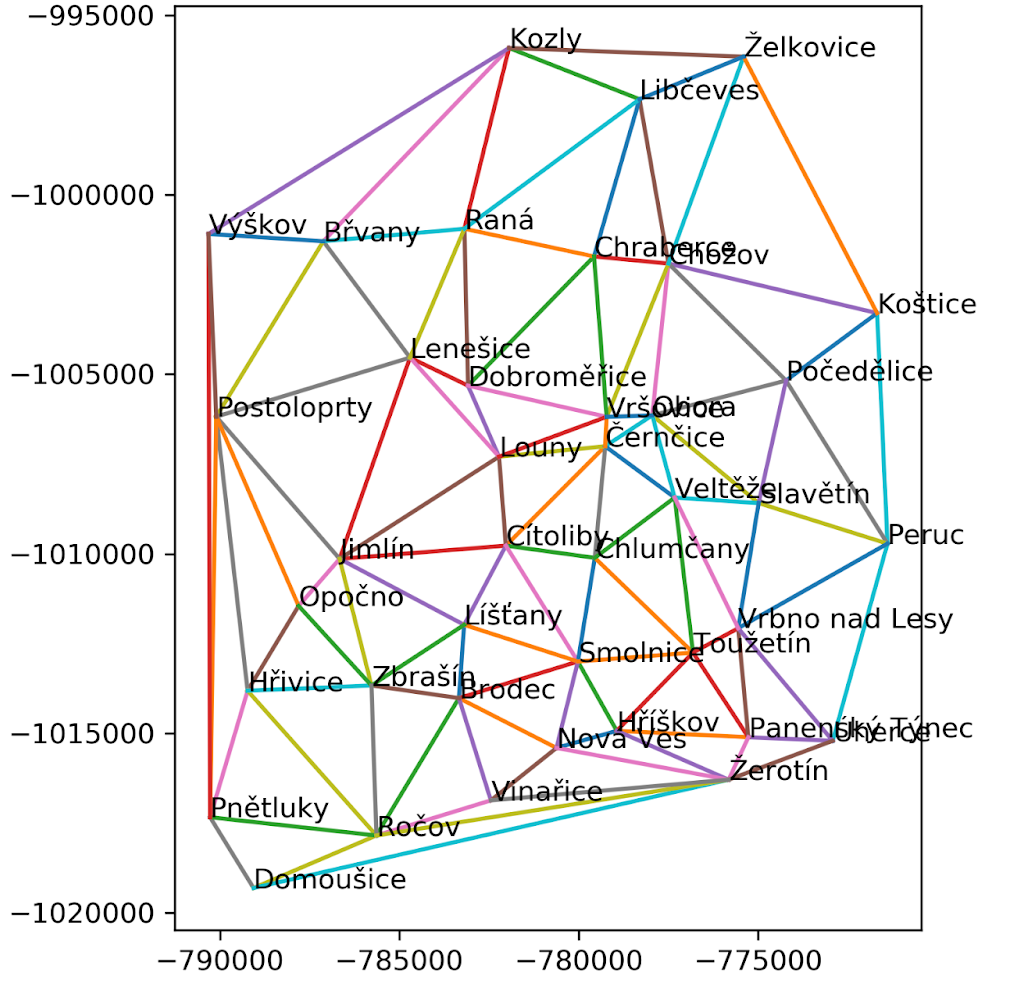
\includegraphics[width=60mm]{pic/doprava_01.png}
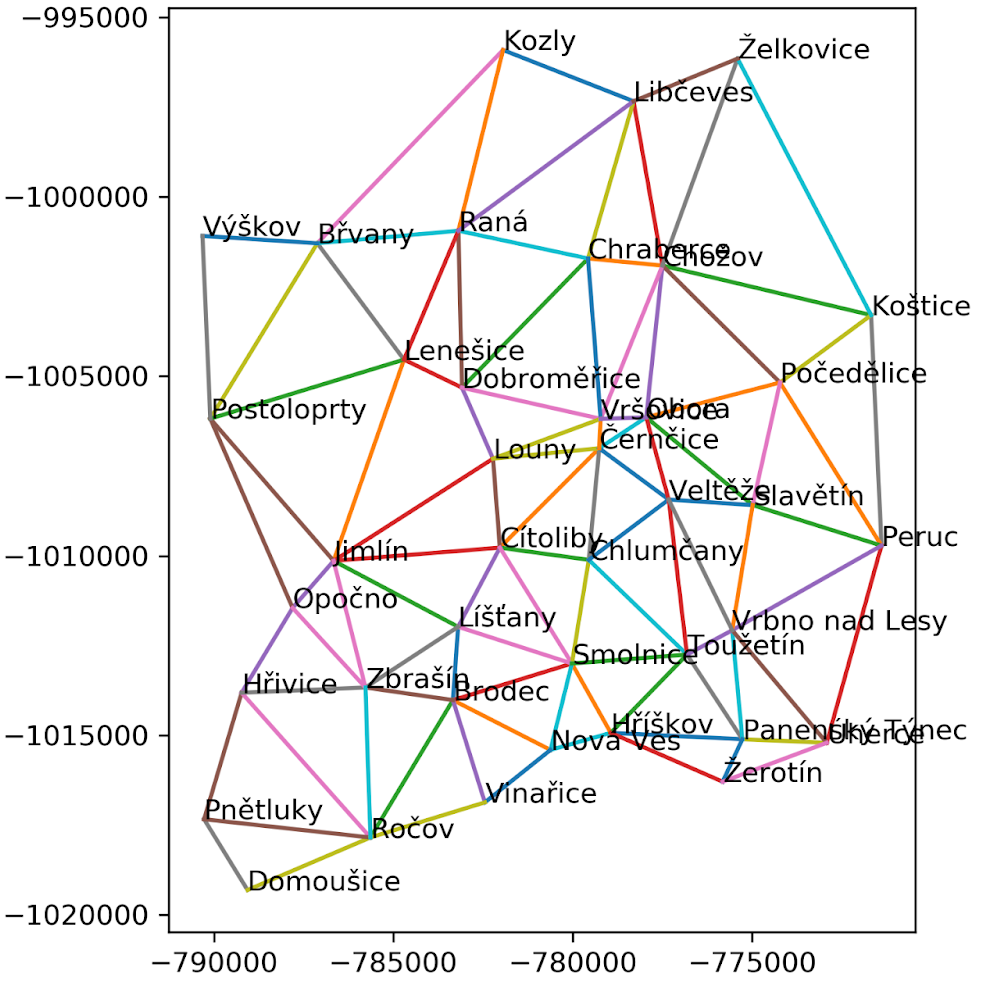
\includegraphics[width=60mm]{pic/doprava_02.png}
\caption{Ukázka úplné a redukované automaticky generované dopravní sítě v~lounském okrese. Vlevo -- úplná síť, vpravo -- síť očištěná o~nadbytečné hrany.}
\label{dopravnisit}
\end{figure}




\section*{Diskuse}

Data použitá pro tvorbu jednotlivých vrstev grafu kontaktů pocházejí z~nejrůznějších zdrojů, což způsobuje rozdílnost jejich bohatosti i kvality. Kromě použití otevřených zdrojů, u~kterých je třeba počítat s~jejich neúplností danou ve většině případů komunitním vznikem (data získává komunita nadšenců a fanoušků dané problematiky podle svých možností) nebo lokálností, ze které plyne různorodost kvality dat z~geografického hlediska, existují i robustní datové zdroje umožňující získání kvalitních datových podkladů. Těmi jsou státem spravované databáze s~údaji o~obyvatelstvu, databáze geografických informačních systémů či data, která jsou soukromým vlastnictvím komerčních firem, například obchodních řetězců. Přístup k~takovým datům je omezen jednak prostřednictvím GDPR, jednak ochotou vlastníků taková data poskytnout a dále cenou, kterou svým datům přikládají v~případě, že s~jejich poskytnutím souhlasí. Vzhledem ke zjednodušením modelu oproti realitě nejsou explicitně uvedeny kontakty v~zájmových a sportovních klubech, setkávání pěveckých sborů a spolu s~nimi rovněž ostatní aktivity podobného druhu. Je zřejmé, že v případě potřeby získání podrobnějšího grafu kontaktů lze graf o~tyto zpřesňující druhy kontaktů doplnit.

Výsledkem sloučení jednotlivých kontaktních vrstev je graf kontaktů. Z~výše uvedeného je zřejmé, že při jeho tvorbě máme k~dispozici velké množství stupňů volnosti, pro jejichž určení není často možné získat empirická data. Jak z~textu vyplývá, důležitým zdrojem vědecky podložených informací je pro nás publikace \cite{Prem_etal2017}, která obsahuje referenční kontaktní matice pro různé typy kontaktů. Můžeme je tedy srovnávat s~kontaktními maticemi našeho modelu. Výsledek tohoto srovnání je vidět na obr. \ref{maticekontaktu}.

\begin{figure}
\begin{center}
\begin{tabular}{|ccc|}
      \hline
      Graf kontaktů & Referenční hodnoty & Histogram kontaktů\\
      \hline
      \hline
      \multicolumn{3}{|c|}{Domácnosti} \\
      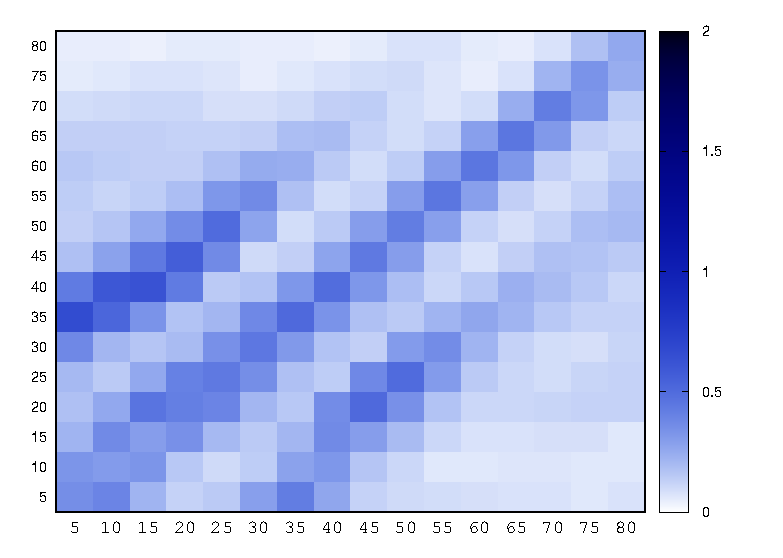
\includegraphics[width=38mm]{pic/home_mat.eps} &
      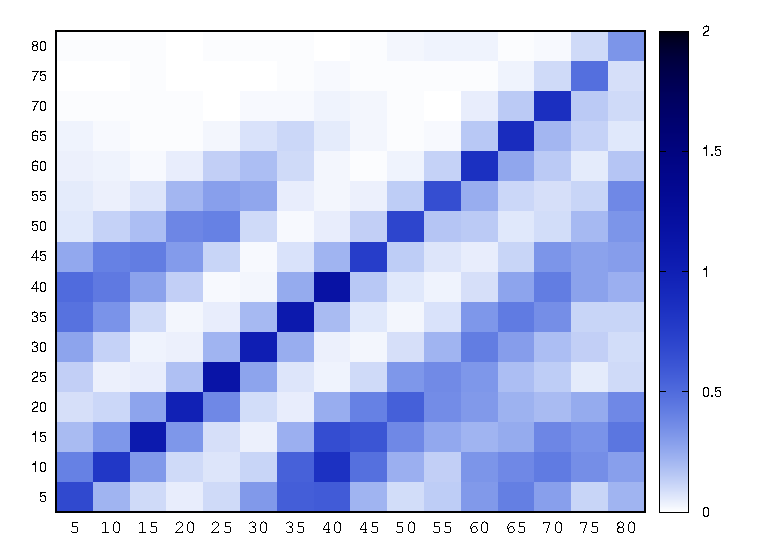
\includegraphics[width=38mm]{pic/home_mat_ref.eps} &
      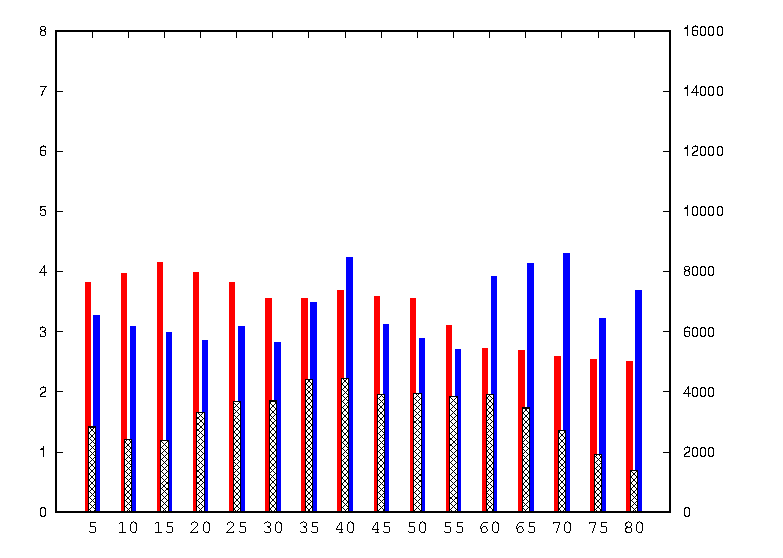
\includegraphics[width=28mm]{pic/home.eps}\\
      \hline
      \multicolumn{3}{|c|}{Zaměstnání} \\
      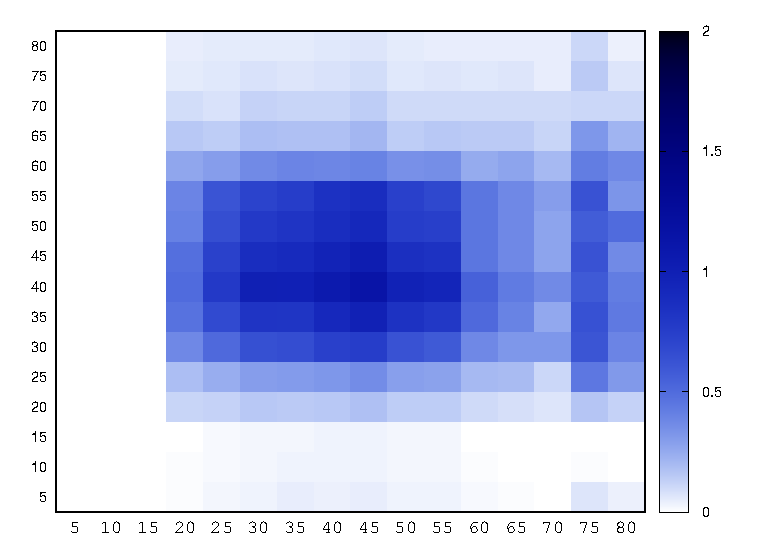
\includegraphics[width=38mm]{pic/work_mat.eps} &
      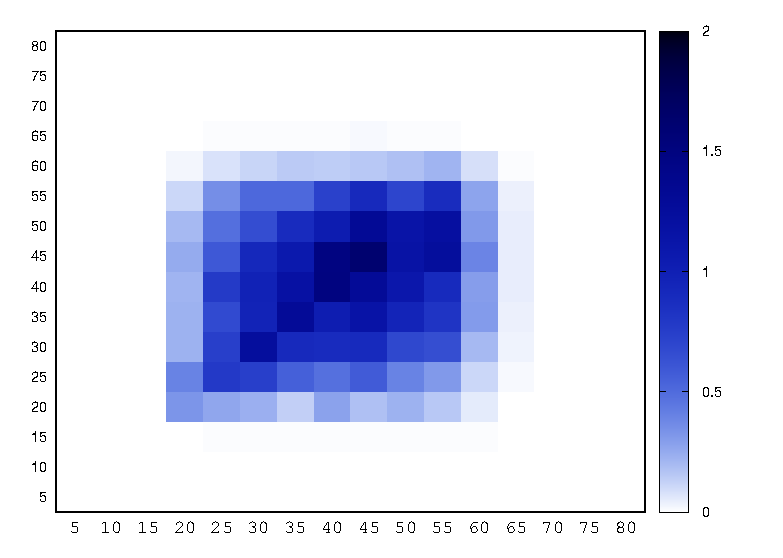
\includegraphics[width=38mm]{pic/work_mat_ref.eps} &
      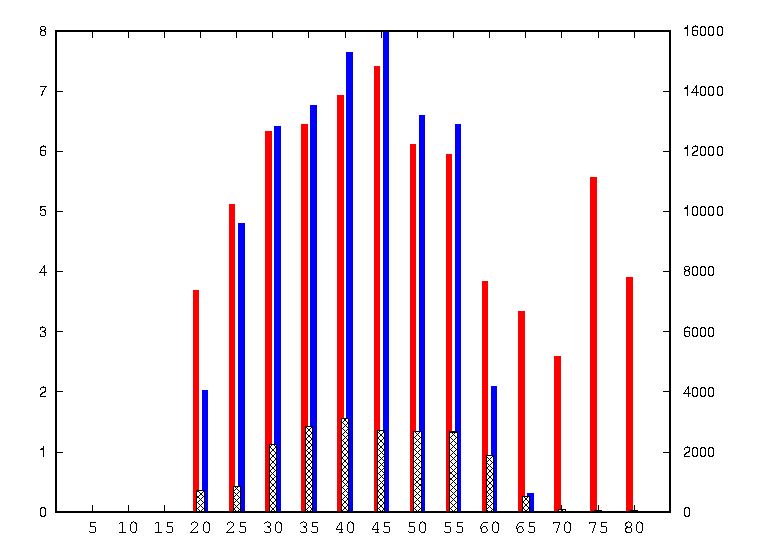
\includegraphics[width=28mm]{pic/work.eps}\\
      \hline
      \multicolumn{3}{|c|}{Školy} \\      
      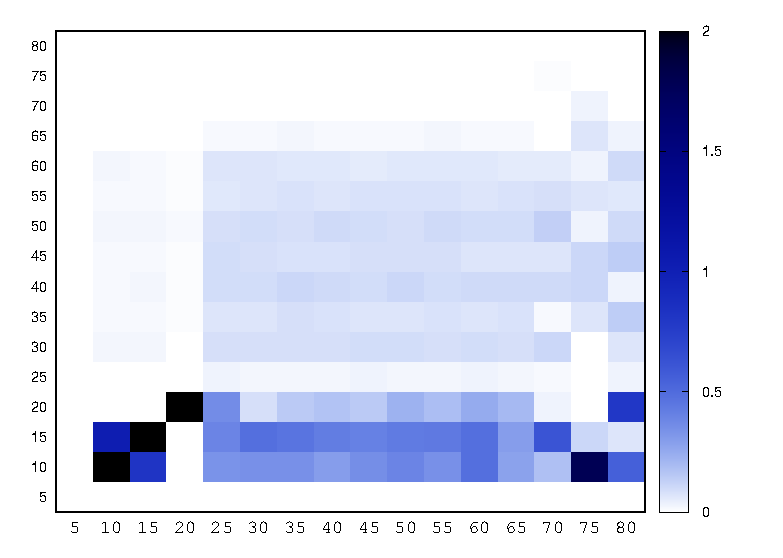
\includegraphics[width=38mm]{pic/school_mat.eps} &
      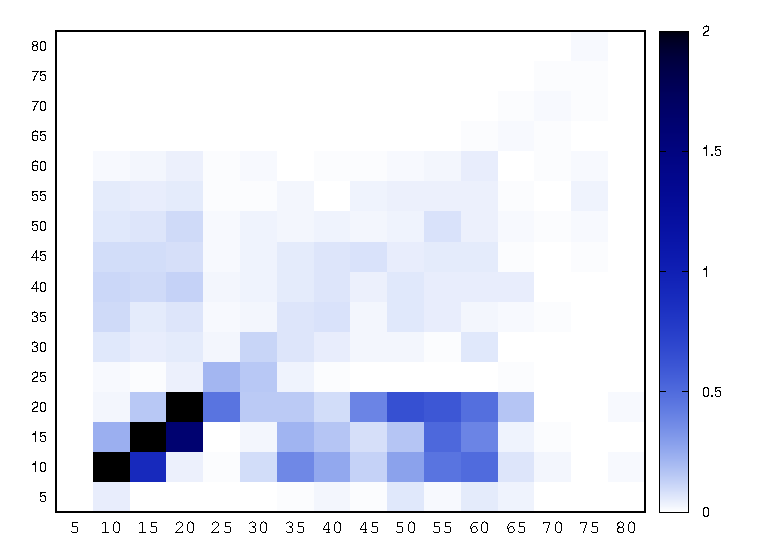
\includegraphics[width=38mm]{pic/school_mat_ref.eps} &
      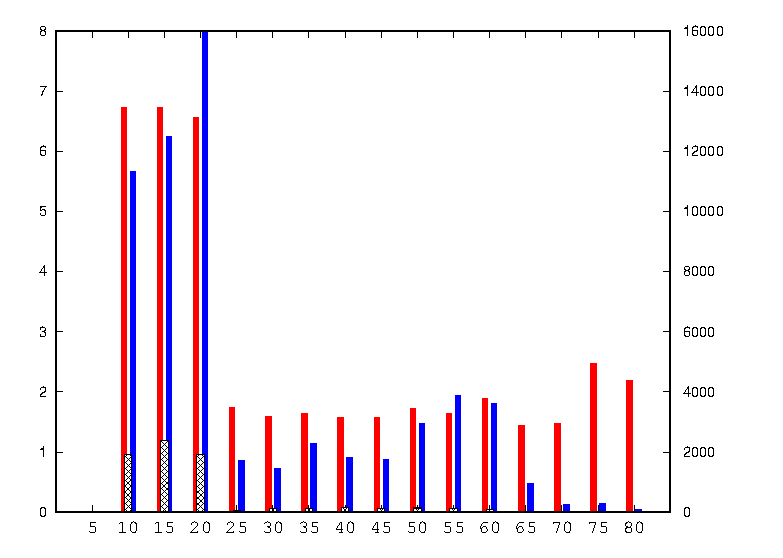
\includegraphics[width=28mm]{pic/school.eps}\\
      \hline
      \multicolumn{3}{|c|}{Ostatní} \\      
      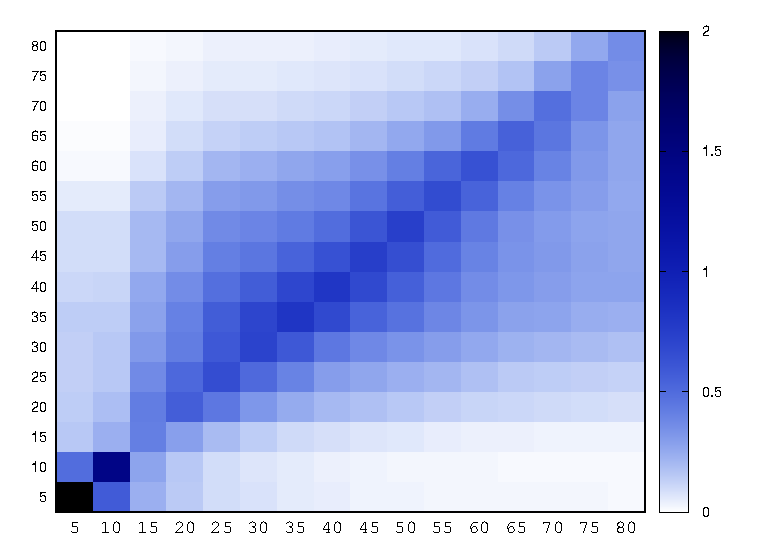
\includegraphics[width=38mm]{pic/other_mat.eps} &
      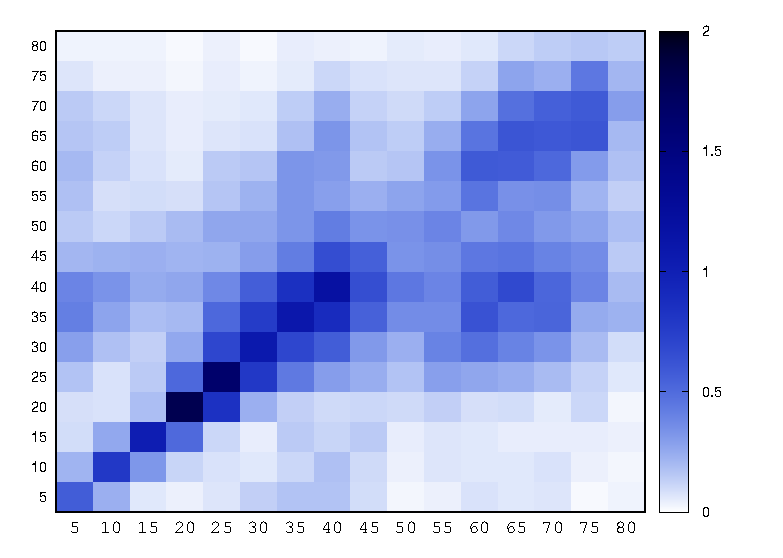
\includegraphics[width=38mm]{pic/other_mat_ref.eps} &
      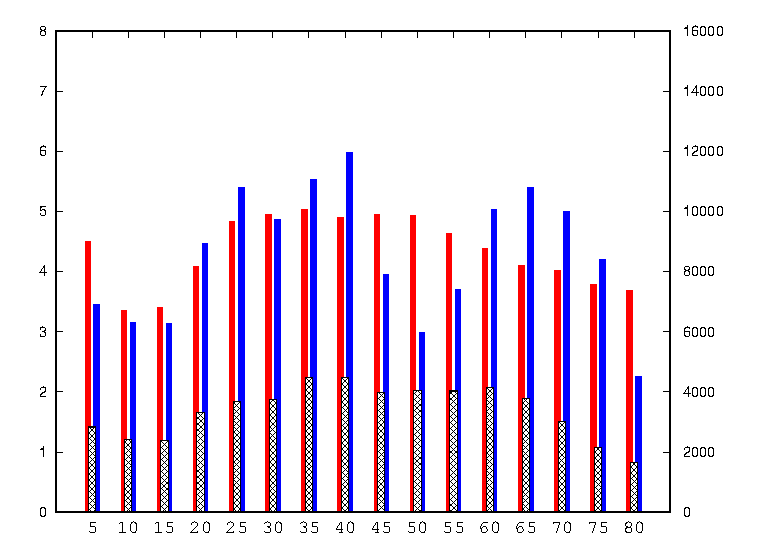
\includegraphics[width=28mm]{pic/other.eps}\\
      \hline
      \multicolumn{3}{|c|}{Všechny kontakty} \\        
      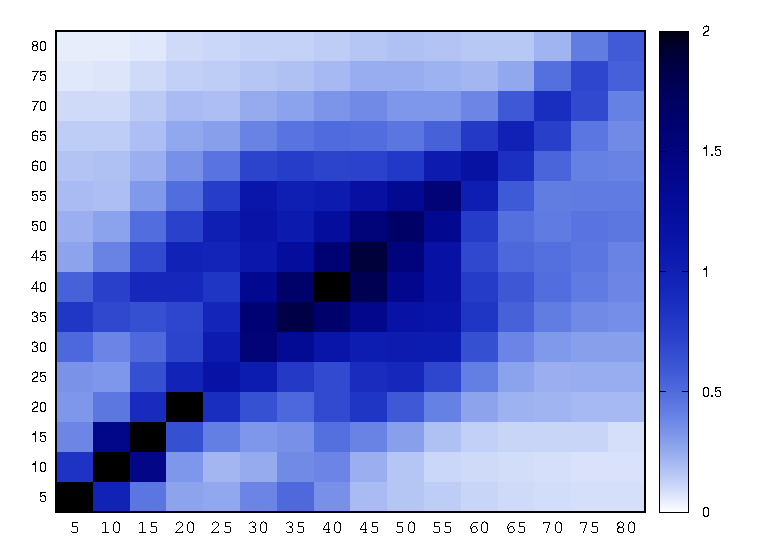
\includegraphics[width=38mm]{pic/all_mat.eps} &
      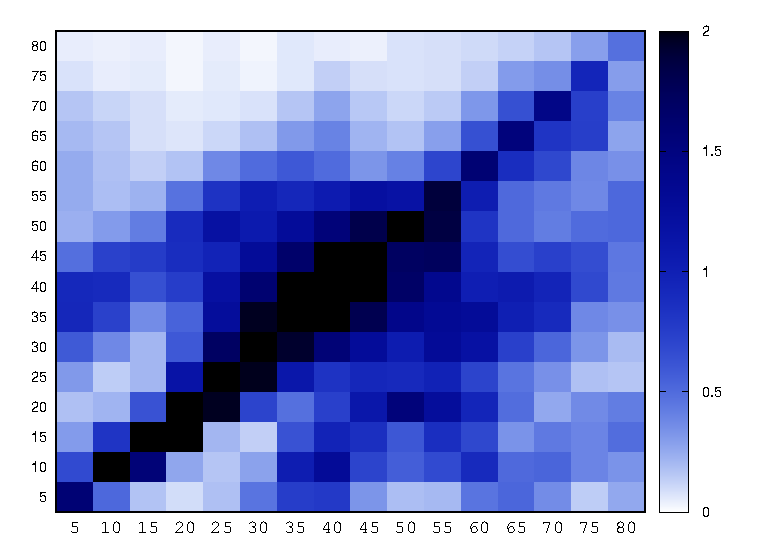
\includegraphics[width=38mm]{pic/all_mat_ref.eps} &
      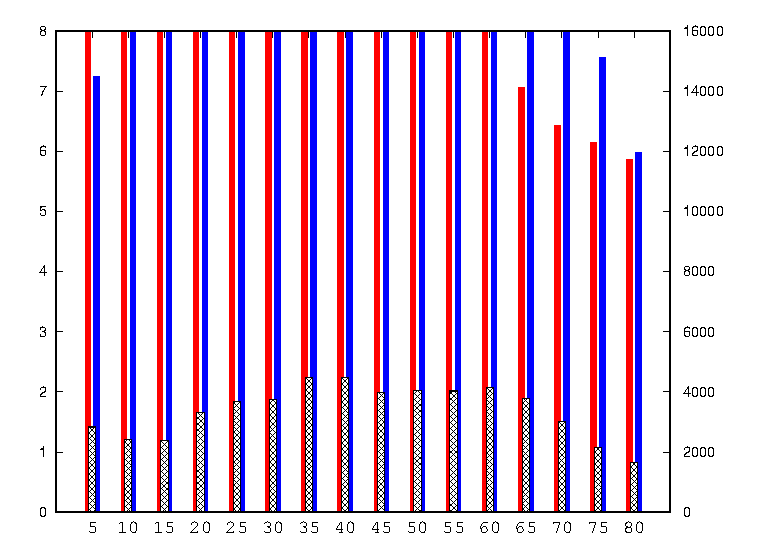
\includegraphics[width=28mm]{pic/all.eps}\\
      \hline

\end{tabular}
\end{center}
\caption{Fitování kontaktů na data.  \\ Levý sloupec: matice kontaktů generovaná z~grafu kontaktů. \\ Prostřední sloupec: referenční matice kontaktů podle \cite{Prem_etal2017}. \\ Pravý sloupec: histogram kontaktů, kde modrá barva označuje hodnoty z~grafu kontaktů, červená barva ukazuje referenční hodnoty a šrafování populaci (váhu).}
\label{maticekontaktu}
\end{figure}

Pro řadu kontaktů však nejsou referenční hodnoty k~dispozici. Matice kontaktů uvedené v~\cite{Prem_etal2017} nemají tak podrobné dělení jako naše kontaktní vrstvy, kterým přisuzujeme váhy tak, aby odpovídaly těmto výzkumům. Nemůžeme si být například jisti množstvím kontaktů v~kategorii přátel, která spadá do referenční kategorie domov (návštěvy) či jiných kategorií. I~když můžeme znát pravděpodobnost návštěvy restaurace pro danou věkovou kategorii, již nezjistíme, kolik restaurací dotyčný navštěvuje. Rovněž znalost poměru venkovních a vnitřních aktivit, která je jistě závislá na počasí, nepochybně hraje při šíření epidemie vý\-znam\-nou roli. Obdobná situace nastává při odhadu počtu návštěvníků obchodů, kde je rozhodně nutné přihlédnout ke skutečnosti, že kontakty v~obchodech jsou většinou krátkodobé.
Velkou otázkou jsou rovněž geografické preference pohybu obyvatel. Ty je možné odhadnout z~hustoty sítě veřejné dopravy. S~dopravou rovněž souvisí pohyb osob mezi regionem a okolím, neboť může významnou měrou ovlivnit výsledek simulace například přílivem pracovních sil z~okolí, nebo naopak jejich odlivem za prací mimo region. Získání dat pro tuto oblast je předmětem dalších aktivit a budou součástí finální verze EPICITY. Jako vhodný zdroj se jeví například anonymizovaná data o~pohybu osob, získaná od operátorů mobilních sítí. 

Jedním z~výhod našeho a podobných modelů je možnost sledovat šíření epidemie regionem. Obrázek \ref{sireniepidemie} ukazuje hypotetický příklad, kdy epidemii nestojí v~cestě žádná omezení. Šedivé body představují zdravé obyvatele, červenou barvou jsou označeni nemocní a černé body reprezentují zemřelé. Vzhledem k~tomu, že modelovaný region je dopravně svázán poměrně hustou dopravní infrastrukturou, dochází k~šíření infekce ve všech sídlech s~obdobnou intenzitou, což je dáno především právě každodenním cestováním obyvatel do zaměstnání, do škol či na nákupy.

\begin{figure}
\begin{center}
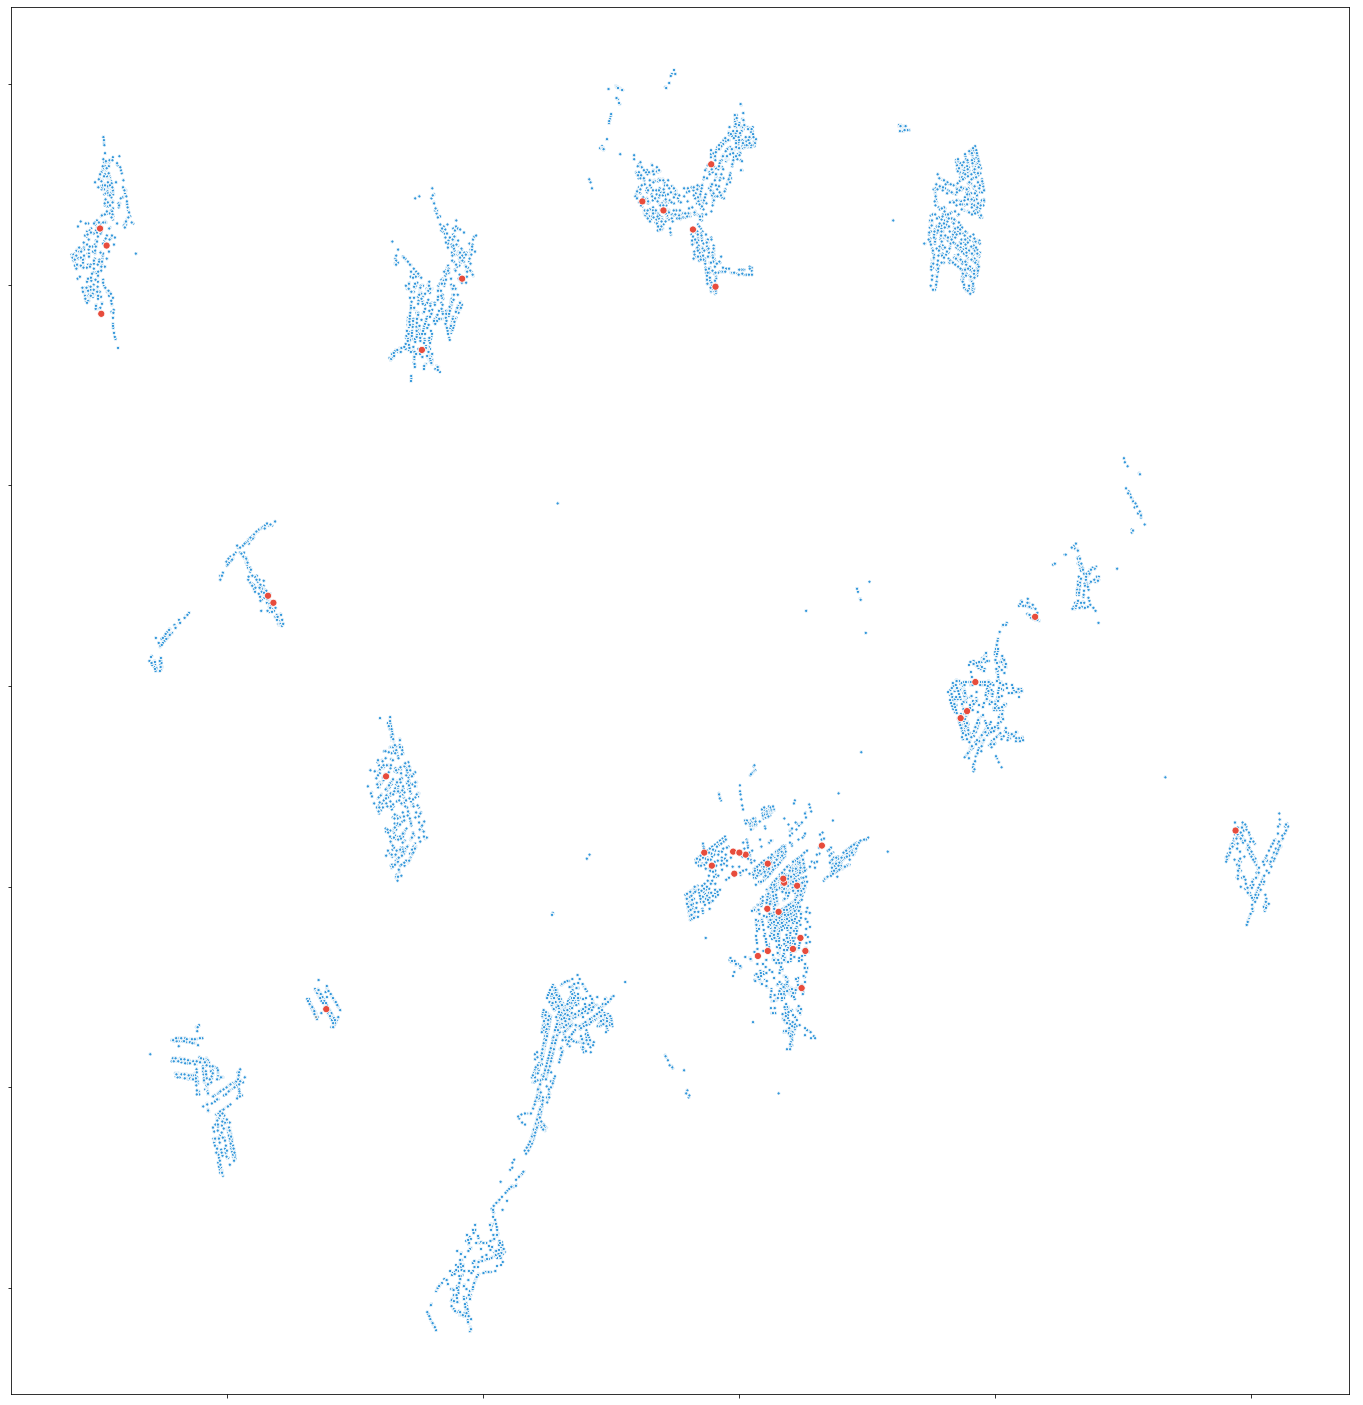
\includegraphics[width=6cm]{pic/hodo002.png}
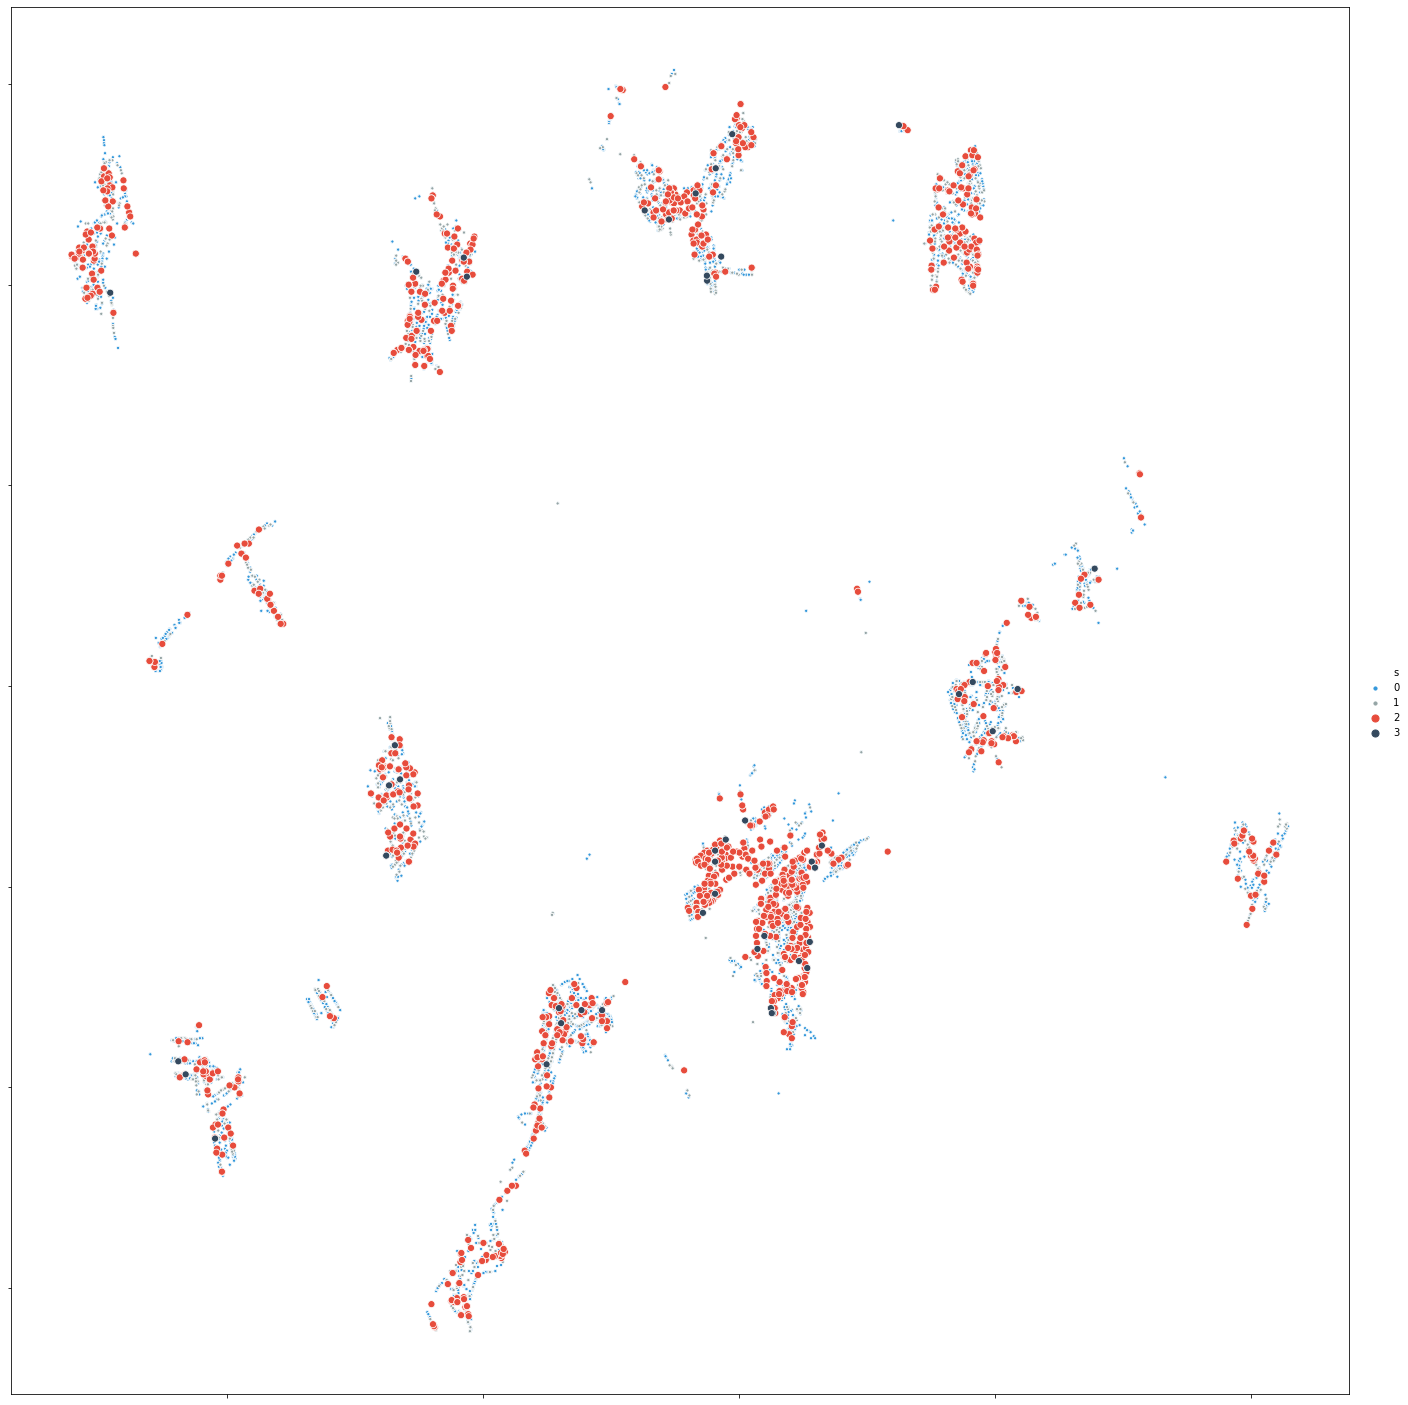
\includegraphics[width=6cm]{pic/hodo180.png}\\
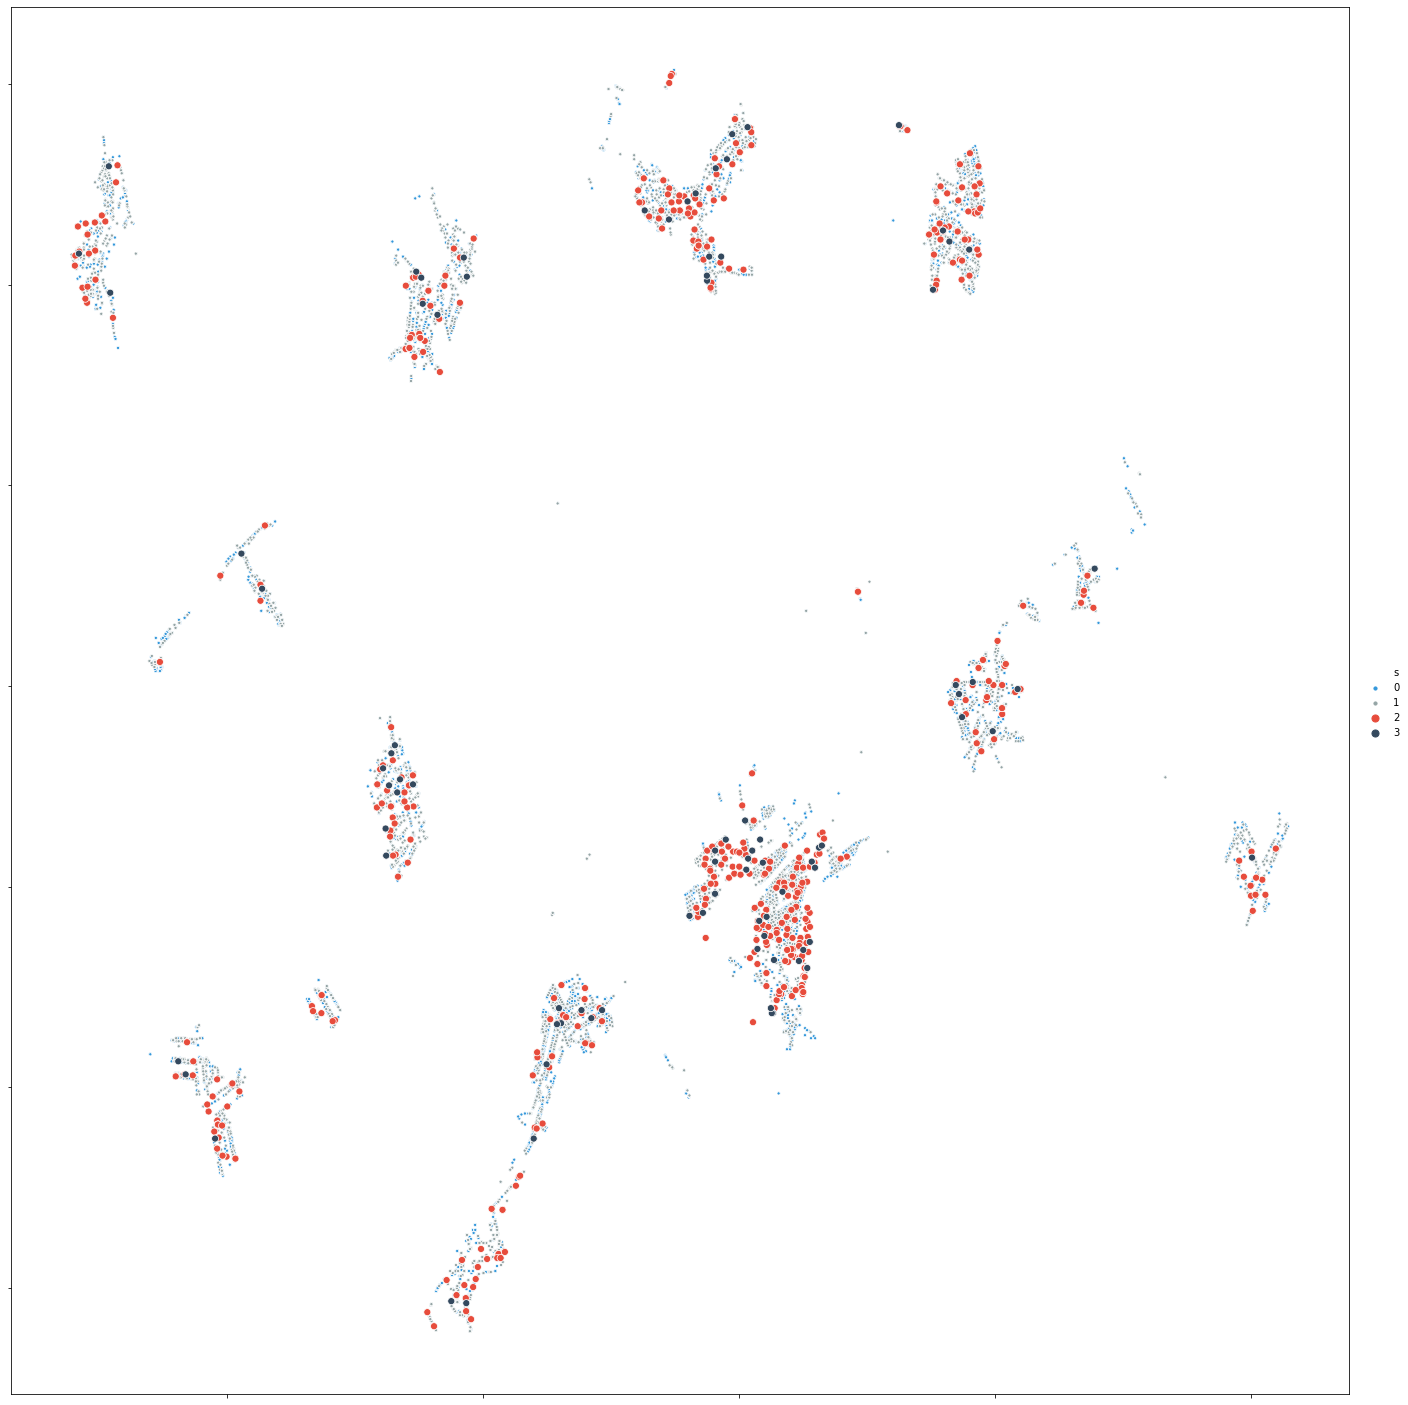
\includegraphics[width=6cm]{pic/hodo295.png}
\end{center}
\caption{Zcela volné šíření epidemie regionem pro 2., 180. a 295. den od počátku simulace. Šedá -- zdraví jedinci, červená -- nemocní, černá -- zemřelí.}
\label{sireniepidemie}
\end{figure}

Praktickým a reálně uplatněným výsledkem, který byl získán díky použití grafu kontaktů adaptovaného pro prostředí konkrétní školy, je odhad vlivu rotační výuky. Jedním z~výsledků je konstatování, že střídání žáků 2. stupně ZŠ i při plném provozu 1. stupně může snížit šíření covid-19 až o~polovinu proti běžnému stavu. Na 1. stupni ZŠ se covid-19 šíří významně méně než na 2. stupni. Podrobně je problematika modelování školního prostředí uvedena v~kapitole \ref{Skoly}. Pro tvorbu grafu kontaktů nebyl v~tomto případě použit automatický generátor, nýbrž bylo v~konkrétní škole provedeno dotazníkové šetření mezi žáky i učiteli \cite{BISOP-VZ-sireni-skoly}. Lze tedy předpokládat větší věrnost takto získaného grafu reálnému stavu.


Jakkoli jsou datové podklady, které používáme, často kusé anebo nedostupné, podrobnou analýzou jednotlivých druhů kontaktů a jejich kombinací je možné získat funkční a v~epidemickém modelu použitelný graf kontaktů vedoucí k~výsledkům odpovídajícím realitě. To lze ukázat například porovnáním predikce vývoje kontaktů našeho modelu s~daty ze sociologických výzkumů (pokud tato data nebyla použita jako vstupy do modelu), daty o~vytíženosti dopravy, počtu návštěvníků restaurací a obchodů a především srovnáním s~epidemickými daty získávanými v~průběhu epidemie. 

Výhodou použití grafu kontaktů, modelujícího až na úroveň jednotlivců, je pře\-de\-vším možnost přisoudit každé osobě konkrétní vlastnosti i způsob chování a sledovat, jakým způsobem se změní výsledky simulace. Každý simulovaný svět, který takto vytvoříme, umožňuje srovnávat hypoteticky možné scénáře chování společnosti s~realitou, která je dána skutečným průběhem epidemie. A~jelikož je do grafu kontaktů možno vložit přesně geograficky i sociálně definované infekční jedince, můžeme zjistit, jakým způsobem se změní šíření epidemie například díky superspreadingovým událostem, ať už jde o~setkání v~restauracích, na sportovních utkáních či v~některé ze škol. 

Z~uvedeného je patrné, že model založený na grafu kontaktů vytvořeném podle zde uvedené metodiky umožňuje vytvářet nejrůznější scénáře situací, jejichž srov\-ná\-ním je možné získat představu o~šíření epidemie za nejrůznějších podmínek. Oproti jiným modelům však tento přístup vyžaduje velké úsilí při získávání potřebných dat a pro jeho vyladění je třeba značných odborných i časových investic.



